
There are various types of robot arms available in the market, some of them can be considered really small in size and suitable for the requirements.
Certain disadvantages exist that are often found in existing models of robot manipulators.





\begin{figure}[H]
	\centering
	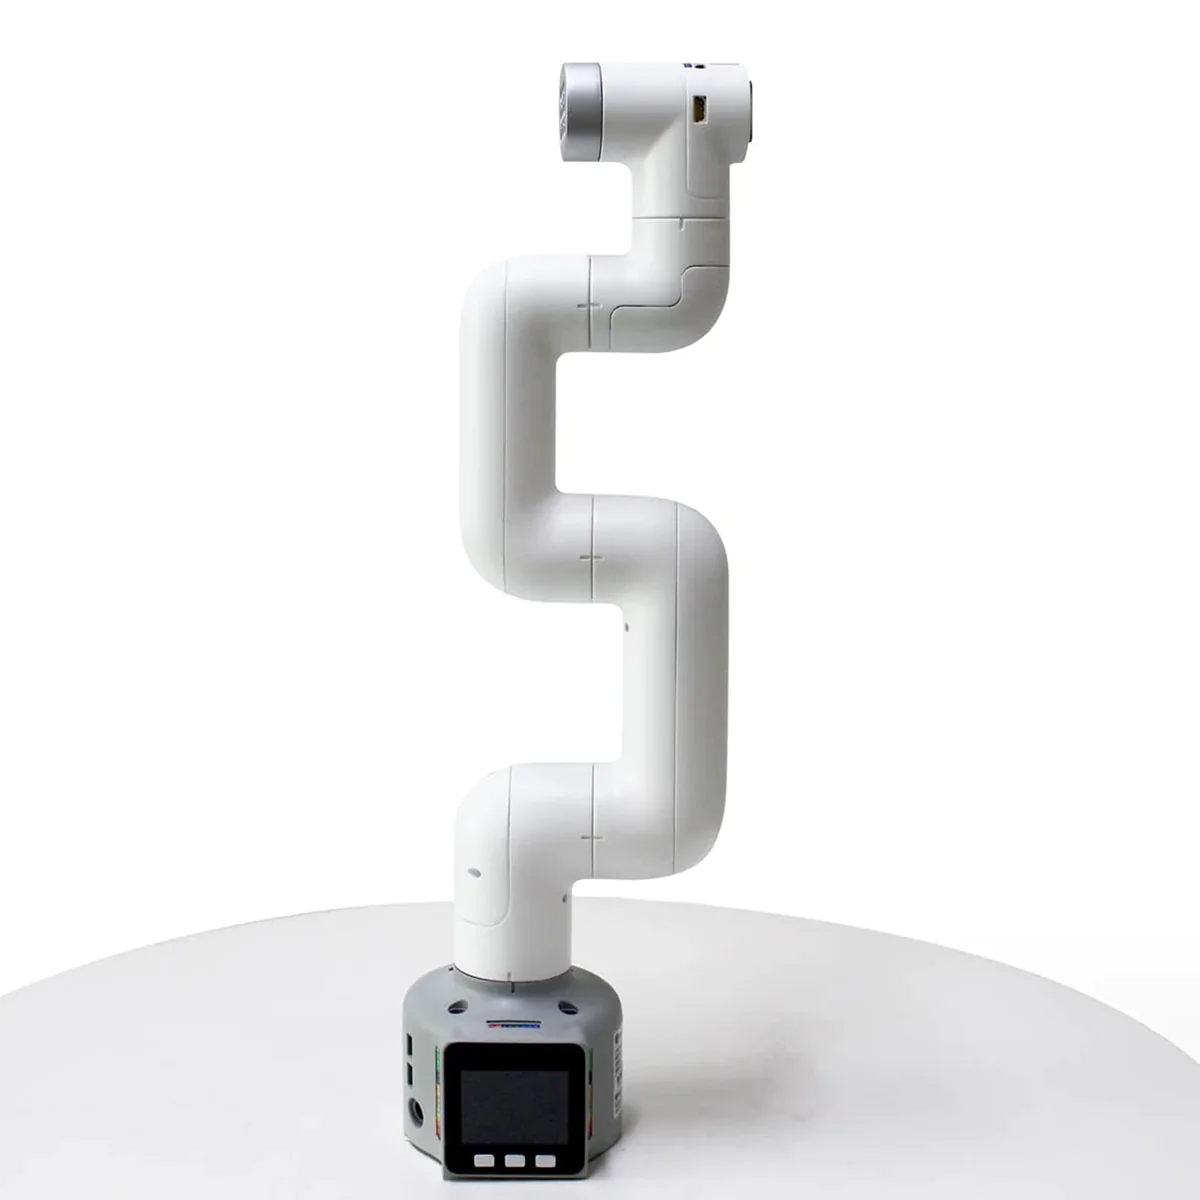
\includegraphics[width=0.4\textwidth]{Src/images/myCobot.png}
	\caption{MyCobot 280}
    \label{mycobot1}
    
\end{figure}
One of the popular models that is available on the market and can be available is the \textbf{myCobot} model robot, shown in the picture \ref*{mycobot1}, as well as technical specifications of the robots represents in the table \ref*{tab:mycobot1}.


\begin{table}[H]
    \caption{Specifications MyCobot Robot Arm}\label{tab:mycobot1}
    \centering
    \begin{tabular}{|l|c|c|}
        \hline
        \textit{\textbf{Parameter ame}} & \multicolumn{1}{l|}{\textit{\textbf{Value}}} & \multicolumn{1}{l|}{\textit{\textbf{Units}}} \\ \hline
        DOF                  & 6     & -     \\ \hline
        Payload              & 0.25  & kg    \\ \hline
        Weight               & 0.8   & kg    \\ \hline
        PRepeatability & ± 0.5 & mm    \\ \hline
        Power Voltage        & DC 12 & V     \\ \hline
        Power Current        & 5     & A     \\ \hline
        Gear type            & -     & Steel \\ \hline
        Shell                & -     & Metal \\ \hline
        Max. reach           & 280     & mm \\ \hline
        Cost                & 800    & Euro \\ \hline
        \end{tabular}
 \end{table}

 


 In most cases, one of the main factors in this type of robot is the use of more low-cost actuators that drive the robot's axis. This may be the use of more low-cost gearboxes and motors that greatly reduce the cost of the entire robot, but the lifetime of these systems is relatively short.

 In the process of testing the basic specifications that was explained that with not all the parameters that are presented in the table \ref*{mycobot1} data are not all reliable, the accuracy of movement is highly dependent on the load at the end of the 6 axis of the robot. Thus, the repeatability of the robot movement was not within \textbf{\pm 0.5 mm}, but could reach deviation around \textbf{ 5 mm}. As shown in figure \ref*{mycobot2} 

 \begin{figure}[H]
	\centering
	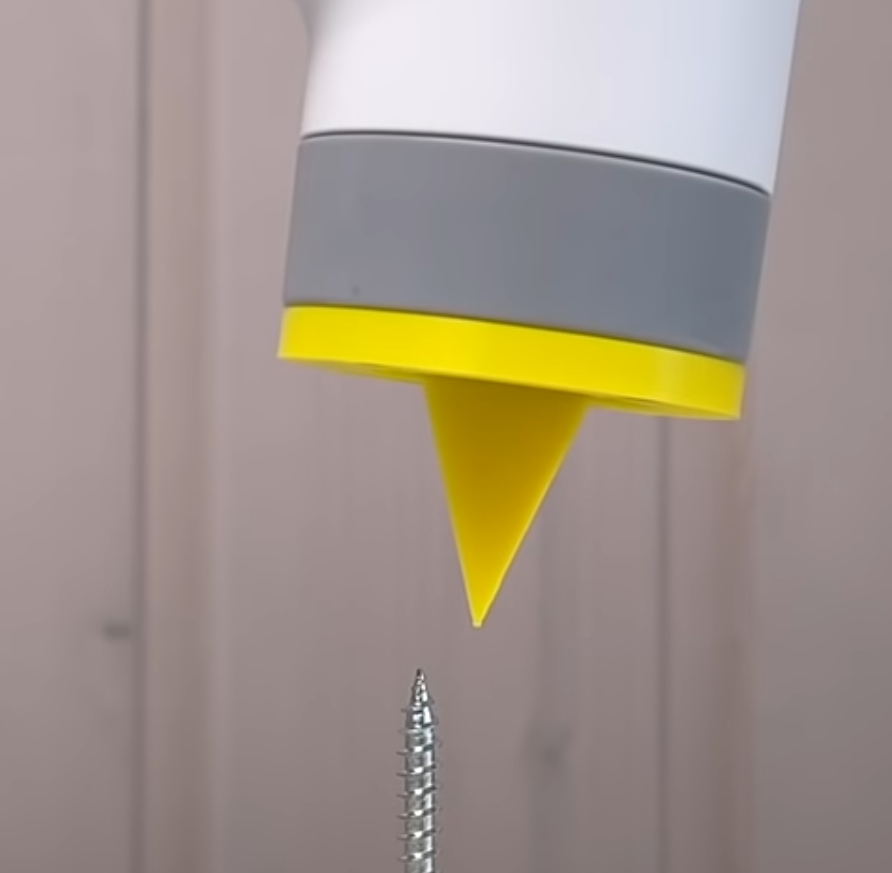
\includegraphics[width=0.4\textwidth]{Src/images/mycobot2.png}
	\caption{Robot repeatability measurement example}
    \label{mycobot2}
\end{figure}

In fact, the servomotors used in hobbyist versions of robotic manipulators, such as the one shown in figure \ref*{mycobot3}, are significantly less accurate and reliable than those used in their industrial counterparts. One of the main reasons for this is that these types of servos are typically designed with cost-effectiveness and basic functionality in mind, rather than high accuracy or durability. This can lead to inconsistent performance, frequent failures and a shorter overall life.


\begin{figure}[H]
	\centering
	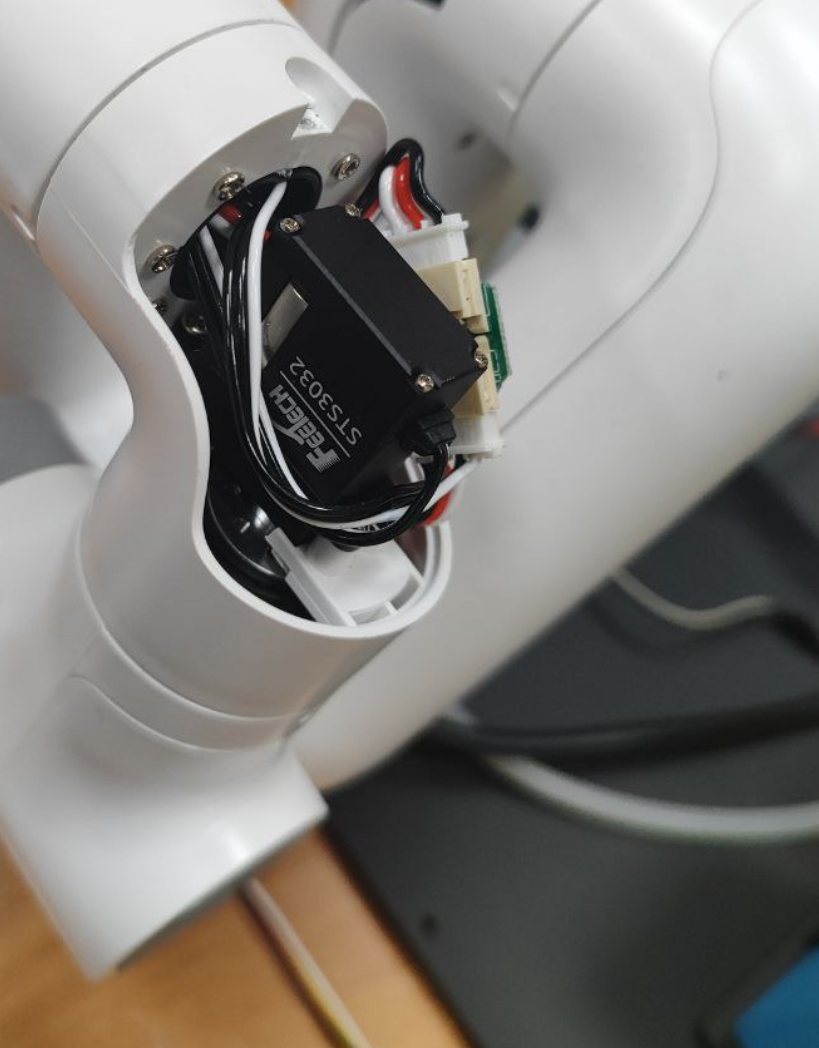
\includegraphics[width=0.4\textwidth]{Src/images/mycobot3.png}
	\caption{Hobbyist Servo Motor}
    \label{mycobot3}
\end{figure}


In addition, the lightweight construction of these servomotors can make them more susceptible to physical impact and other environmental factors. This lack of robustness often results in frequent maintenance, which can lead to increased downtime and reduced productivity.

Hobbyist servomotors often have less sophisticated control systems, which may not provide the advanced features required for precise control in complex applications. 

 \begin{figure}[H]
	\centering
	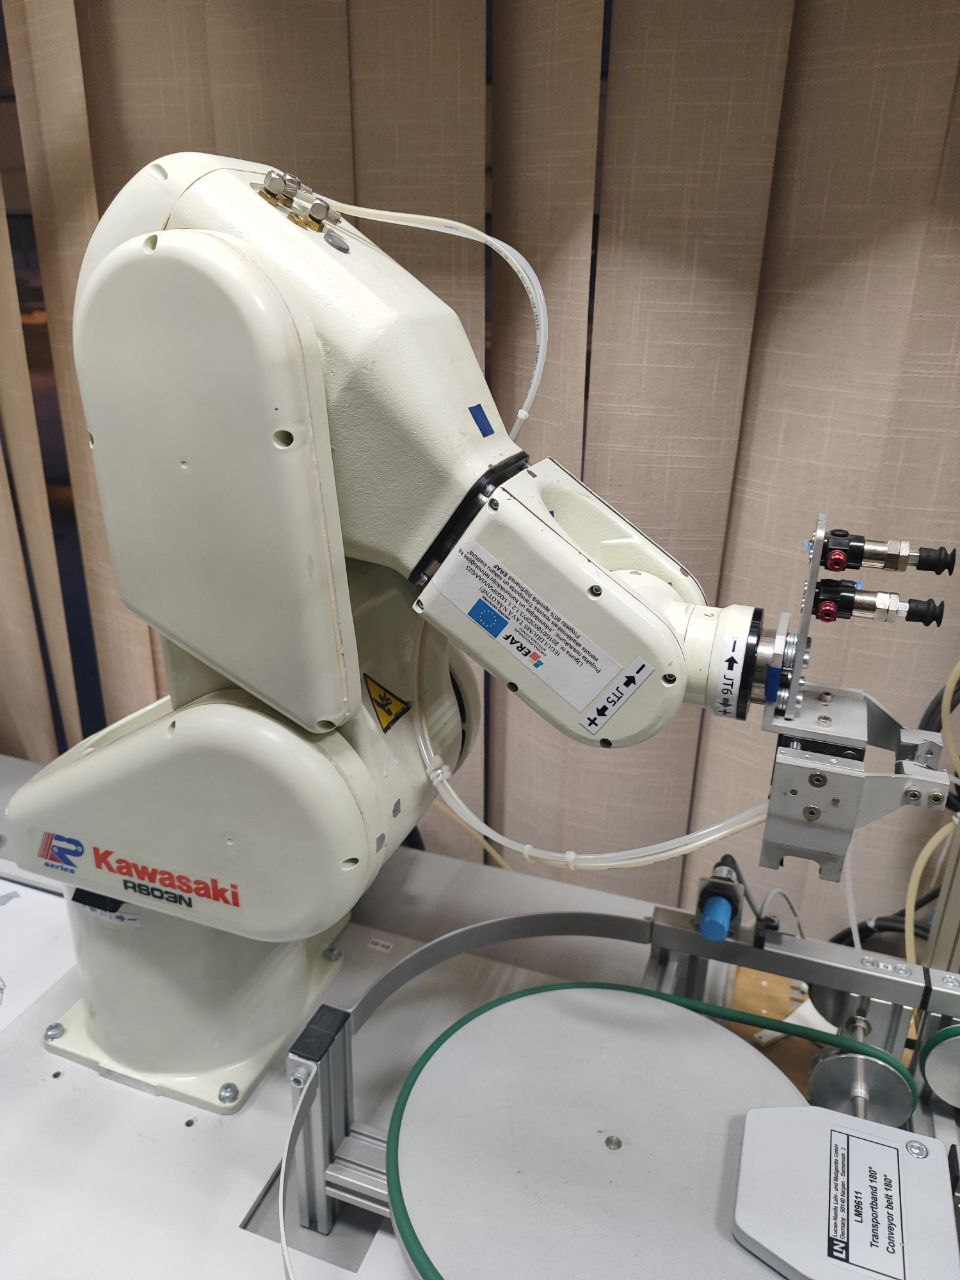
\includegraphics[width=0.6\textwidth]{Src/images/FS03N.jpg}
	\caption{Kawasaki FS03N}
    \label{Kawasaki1}
\end{figure}

\begin{table}[H]
    \caption{Specifications Kawasaki Robot Arm FS03N}\label{tab:Kawasaki1}
    \centering
    \begin{tabular}{|l|c|c|}
        \hline
        \textit{\textbf{Parameter ame}} & \multicolumn{1}{l|}{\textit{\textbf{Value}}} & \multicolumn{1}{l|}{\textit{\textbf{Units}}} \\ \hline
        DOF                  & 6     & -     \\ \hline
        Payload              & 3 & kg    \\ \hline
        Weight               & 20   & kg    \\ \hline
        Repeatability        & ± 0.02 & mm    \\ \hline
        Power Voltage        & AC 230 & V     \\ \hline
        Max Power Current    & 9    & A     \\ \hline
        Gear type            & -     & Steel \\ \hline
        Shell                & -     & Aluminium \\ \hline
        Max. reach           & 620     & mm \\ \hline
        Cost                & 12 000     & Euro \\ \hline
        \end{tabular}
 \end{table}

 
\begin{figure}[H]
	\centering
	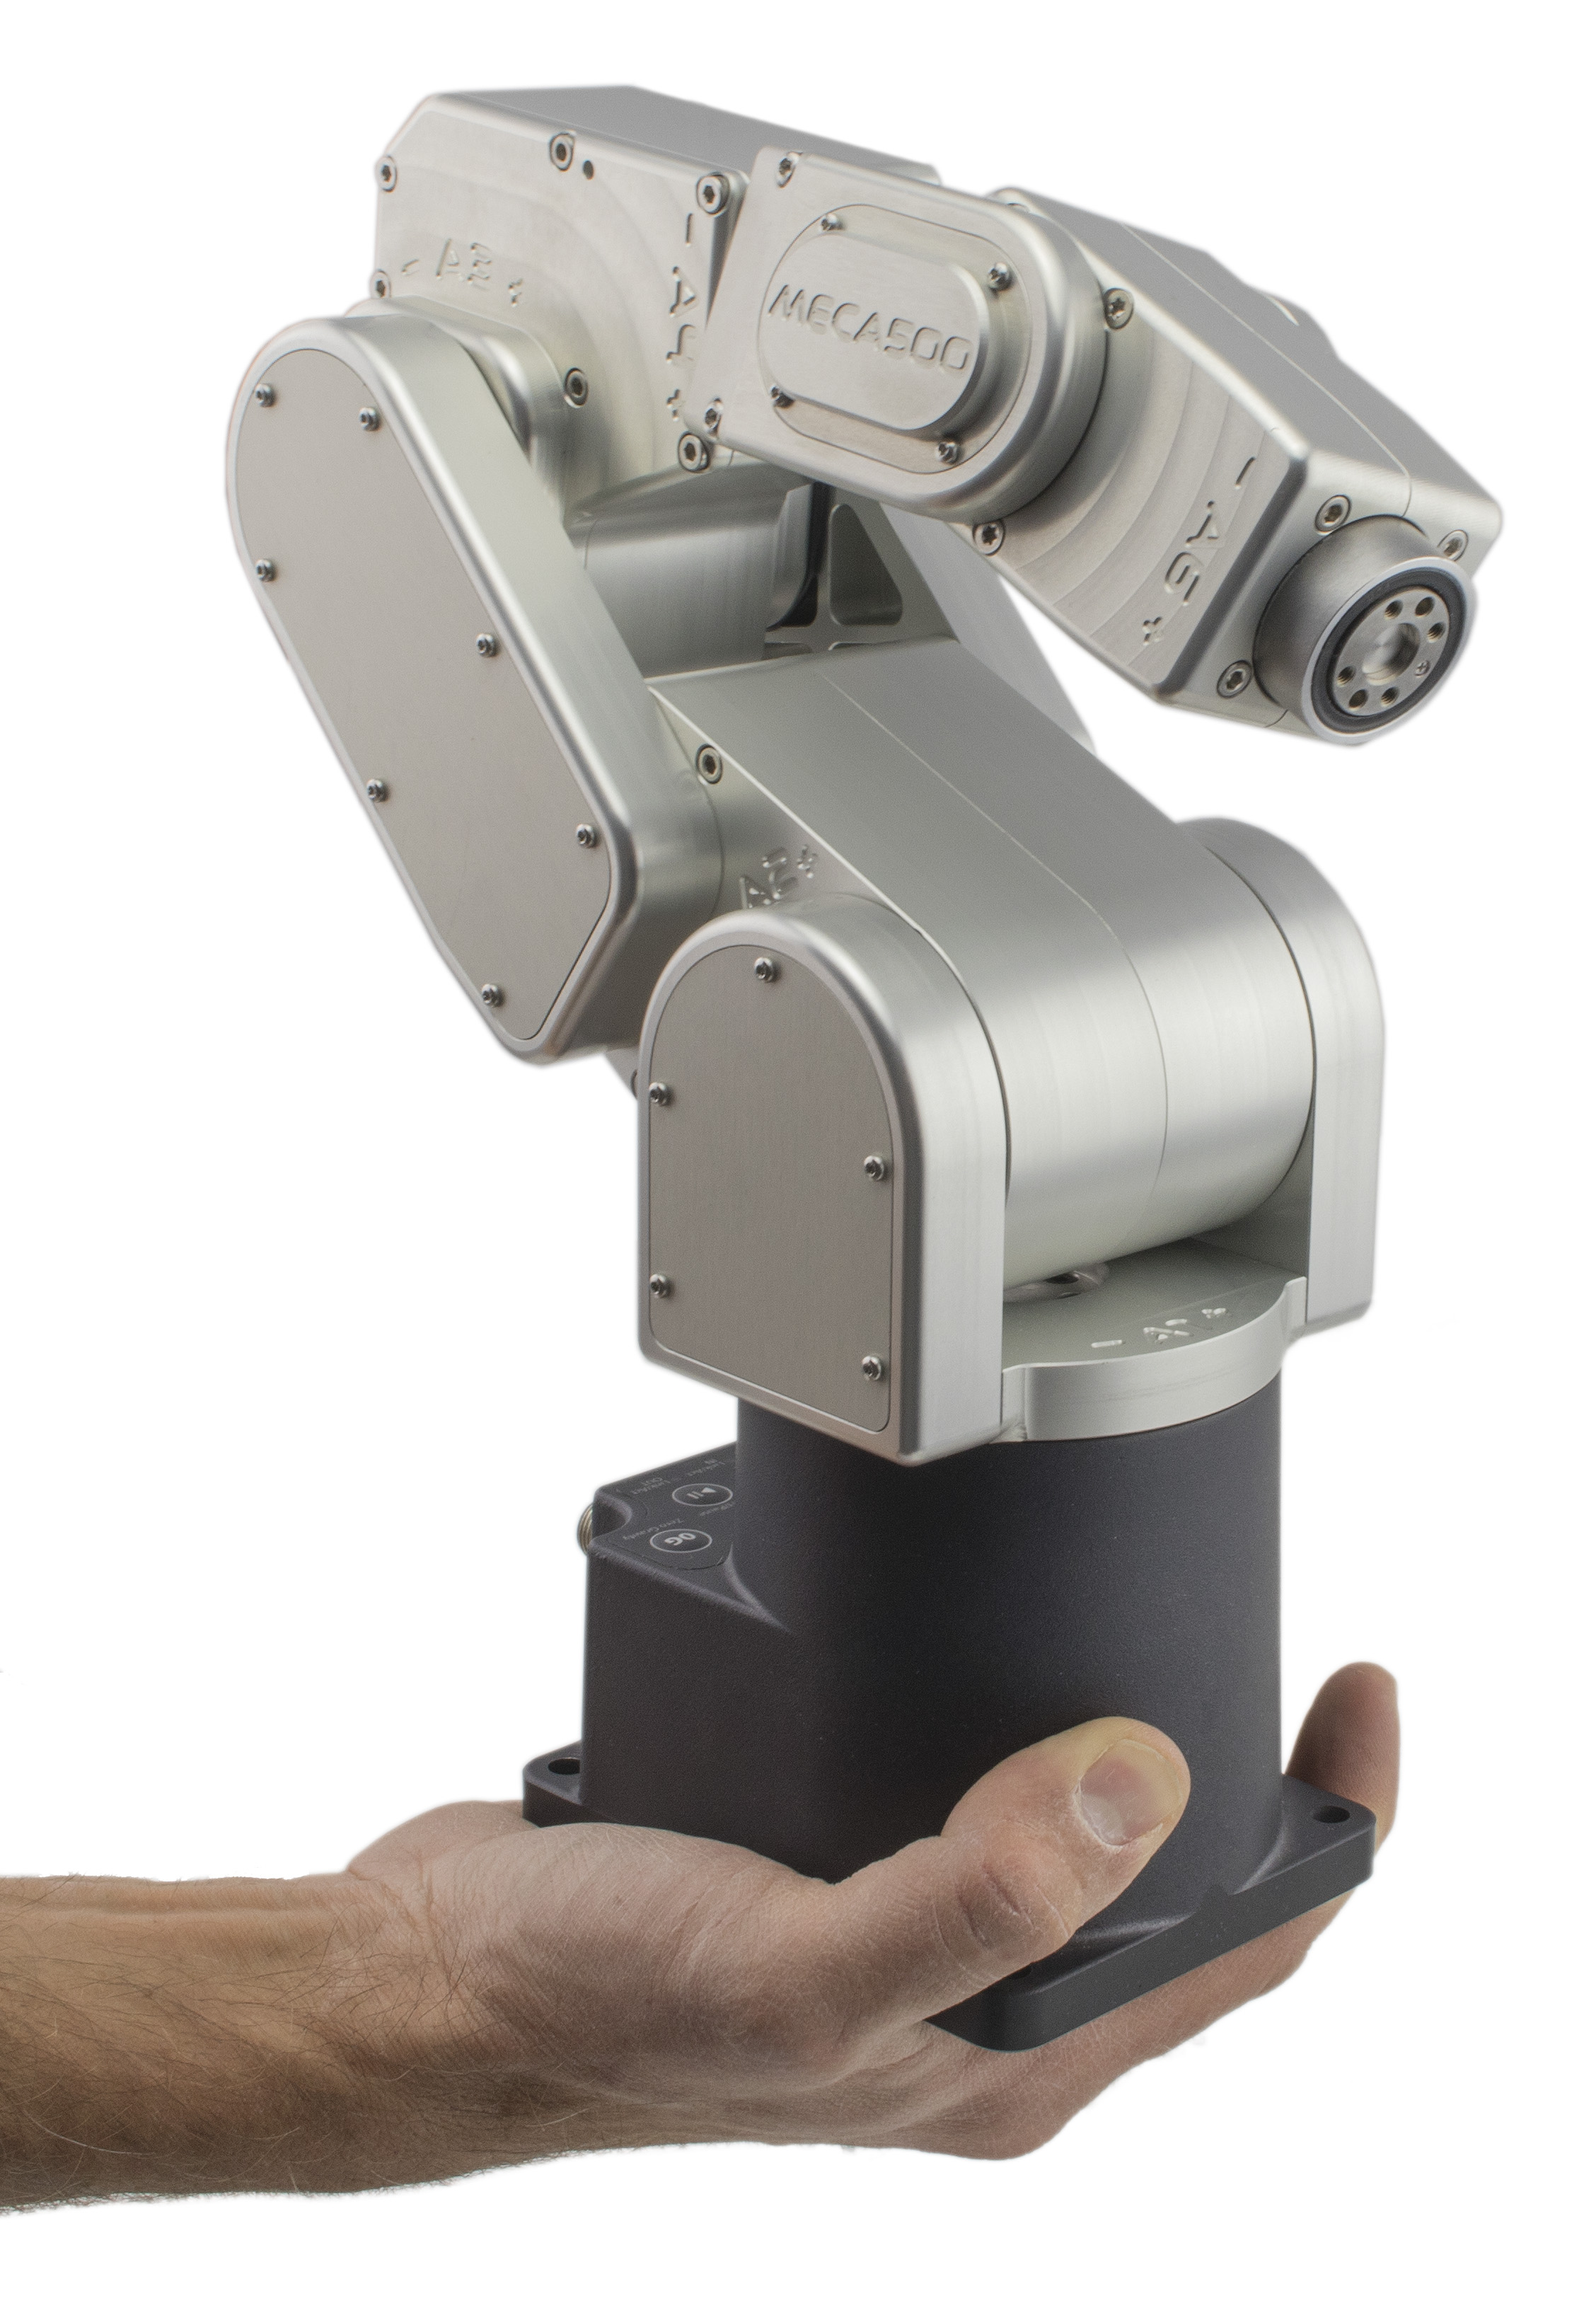
\includegraphics[width=0.4\textwidth]{Src/images/Meca500.jpg}
	\caption{Meca 500}
    \label{Meca1}
\end{figure}

\begin{table}[H]
    \caption{Specifications for Meca 500 Robot Arm}\label{tab:Meca1}
    \centering
    \begin{tabular}{|l|c|c|}
        \hline
        \textit{\textbf{Parameter ame}} & \multicolumn{1}{l|}{\textit{\textbf{Value}}} & \multicolumn{1}{l|}{\textit{\textbf{Units}}} \\ \hline
        DOF                  & 6     & -     \\ \hline
        Payload              & 0.5 & kg    \\ \hline
        Weight               & 4.5   & kg    \\ \hline
        PRepeatability & ± 0.005 & mm    \\ \hline
        Power Voltage        & DC 24 & V     \\ \hline
        Max Power Current        & 9    & A     \\ \hline
        Gear type            & -     & Steel \\ \hline
        Shell                & -     & Aluminium \\ \hline
        Max. reach           & 330     & mm \\ \hline
        Cost                & 12 000     & Euro \\ \hline
        \end{tabular}
 \end{table}